%
% File acl2010.tex
%
% Contact  jshin@csie.ncnu.edu.tw or pkoehn@inf.ed.ac.uk
%%
%% Based on the style files for ACL-IJCNLP-2009, which were, in turn,
%% based on the style files for EACL-2009 and IJCNLP-2008...

%% Based on the style files for EACL 2006 by 
%%e.agirre@ehu.es or Sergi.Balari@uab.es
%% and that of ACL 08 by Joakim Nivre and Noah Smith
\PassOptionsToPackage{xetex}{xcolor}
\documentclass[11pt]{article}
\usepackage[hidelinks]{hyperref,xcolor}
\hypersetup{
     colorlinks,
     linkcolor={blue!50!black},
     citecolor={red!50!black},
     urlcolor={blue!80!black}
}
\usepackage[round]{natbib}

\usepackage{polyglossia}
\setmainlanguage{english}
\setotherlanguage{urdu}
%\setotherlanguage{myanmar}
%\setmainfont[Mapping=tex-text]{Times New Roman}
\usepackage{xeCJK}
%\setCJKmainfont{WenQuanYi Micro Hei}
% \setmainfont[Numbers=OldStyle]{TeX Gyre Pagella}
%\setCJKmainfont{Droid Sans Fallback}
\setCJKmainfont{Noto Sans CJK SC}
\setCJKsansfont{Noto Sans CJK SC}
%\setmainfont{Noto Sans}
\newfontfamily\urdufont[Script=Arabic,Language=Urdu,Scale=1.5]{Amiri}
% or Scheherazade after installing the font
%sudo apt-get install font-hosny-amiri
\newfontfamily\myanmarfont[Script=Myanmar]{Padauk}
\newcommand{\myanmar}[1]{{\myanmarfont #1}}
\usepackage{acl2010}
\newcommand{\secref}[1]{\StrSubstitute{\getrefnumber{#1}}{.}{ }}

\setmainfont{Noto Serif}%TeX Gyre Termes}

\usepackage[j,e]{mtg2e}
\usepackage{mygb4e}
\usepackage{url}
\usepackage{latexsym}
\usepackage{graphicx}
\usepackage{enumitem}
\usepackage{omwmacros}
%\setlength\titlebox{6.5cm}    % You can expand the title box if you
% really have to

\newcommand{\lex}[1]{\textbf{\textit{#1}}}
\title{Linking the TUFS Basic Vocabulary \\ to the Open Multilingual Wordnet}

\author{
	Francis Bond,$^\spadesuit$ 
	Hiroki Nomoto ,$^\diamondsuit$
	Luis Morgado da Costa$^\spadesuit$\\
  $^\spadesuit$ Nanyang Technological University (NTU),  Singapore\\
  $^\diamondsuit$
  Tokyo University of Foreign Studies (TUFS), Japan \\
  \url{bond@ieee.org, nomoto@tufs.ac.jp} }

\date{}

\begin{document}
\maketitle
\begin{abstract}
We describe the linking of the TUFS Basic Vocabulary Modules, created for
on-line language learning, with the Open Multilingual Wordnet.  The
links are then used to (i) evaluate existing wordnets, (ii) add data
to these wordnets and (iii) create new open w1ordnets for Khmer,
Korean, Lao, Mongolian, Russian, Tagalog, Urdu and Vietnamese.
% Turkish, German, Myanmar


\end{abstract}
\section{Introduction}




Preliminary values for the coverage are shown in Table~\ref{tab:cover}.

\begin{table*}
  \centering
  \begin{tabular}{llrrrl} 
Language& & Concepts	& Words & \% in WN & Comment \\
\hline 
Arabic & ar	& 2,043	& 2,928 & 3\\
Arabic in Syria & as	& 1,184	& 1,053 & 30\\
German & de	&   521	& 1,221 & 0\\
English & en	&   525	& 1,255 & 59\\
Spanish & es	&   587	& 1,207 & 49\\
French & fr	&   969	& 2,076 & 73\\
Indonesian & id	&   621	&   899 & 84\\
Japanese & ja	&   829	& 1,945 & 47\\
Central Khmer & km	&   517	&   465 & 0\\
Korean & ko	&   527	& 1,011 & 0\\
Lao & lo	&   526	&   492 & 0\\
Mongolian & mn	&   553	&   497 & 0\\
Malay & ms	&   829	&   829 & 61\\
Burmese & my	&   829	&   829 & 0\\
Por. in Brazil & pb	&   527	& 1,238 & 72\\
Portuguese & pt	&   519	&   477 & 84\\
Russian & ru	&   556	& 1,102 & 0\\
Thai & th	&   520	&   469 & 80\\
Tagalog & tl	&   525	& 1,195 & 0\\
Turkish & tr	&   537	& 1,959 & 0\\
Urdu & ur	&   755	&   669 & 0\\
Vietnamese & vi	&   629	&   723 & 0\\
Mandarin Chinese & zh	&   596	&   556 & 66\\
Total	&16,224	&25,095 \\
\end{tabular}

  \caption{Wordnet coverage of the basic vocabulary}\label{tab:cover}
\end{table*}


\subsection{TUFS Open Language Resources}


The data comes from the basic vocabulary words and example sentences
in 24 languages in the TUFS Open Language Resources
\citep{Kawaguchi:2007}.  These have also been used as a basis for the TUFS Asian Language
Parallel Corpus, or TALPCo \citep{}.

Nomoto, Hiroki, Kenji Okano, David Moeljadi and Hideo Sawada. 2018. TUFS Asian Language Parallel Corpus (TALPCo). Proceedings of the Twenty-Fourth Annual Meeting of the Association for Natural Language Processing, 436-439.
(For Thai and Vietnamese translations, and interpersonal meaning annotations)
Nomoto, Hiroki, Kenji Okano, Sunisa Wittayapanyanon and Junta
Nomura. 2019. Interpersonal meaning annotation for Asian language
corpora: The case of TUFS Asian Language Parallel Corpus
(TALPCo). Proceedings of the Twenty-Fifth Annual Meeting of the
Association for Natural Language Processing, .
Kawaguchi, Yuji. 2007. Foundations of Center of Usage-Based Linguistic
Informatics (UBLI). In Yuji Kawaguchi, Toshihiro Takagaki, Nobuo
Tomimori and Yoichiro Tsuruga (eds.) Corpus-Based Perspectives in
Linguistics, 3-28. Amsterdam: John Benjamins.

https://github.com/matbahasa/TALPCo

The Japanese component consists of 799 basic vocabulary words with
example sentences for them. These basic vocabulary words were selected
in accordance with the lowest level of the Japanese Language
Proficiency Test, i.e. N5 (equivalent to Level 4 in the old
system). The example sentences are given in a formal conversational
register.  Some of the vocabulary is a little old fashioned (for
example 万年筆 \jpn[fountain pen]{mannenhitu} or フィルム 
\jpn[(photgraphic) film]{firumu}).   We give the translations
for 先生 \jpn[teacher]{sensei} in Table~\ref{tab:teacher}.  We see
here that different languages offer extra information as free text: German, French and Vietnamese have male and
female versions: Russian differentiates school and university
teachers.  Further, Arabic offers irregular plurals and Chinese pinyin
transliterations.\marginpar{translate}

\begin{table*}
  \centering
\begin{tabular}{lll}
Language	&  Cleaned	& Meaning \\ \hline
Arabic (ar)	&	أُسْتَاذٌ	& [名詞]教授(職名)、先生(呼称)أَسَاتِذَةٌ√أستاذ
أستاذ,استاذ,أساتذة,اساتذة \\
Arabic in Syria (as)	& إستاذ (brk:أساتذة)     & 先生 \\
German (de)	    & Lehrer	& 先生,教師 <女>Lehrerin\\
English (en)	    & teacher	& 先生\\
Spanish (es)	    & profesor	& 先生\\
French (fr)		& instituteur	& 先生。とくに小学校の先生。;*女性形はinstitutrice。\\
French (fr)		& professeur	& 先生。教授。;*男女とも同じ形。\\
French (fr)		& enseignant	& 先生。教員。職業としての先生。\\
Indonesian (id)	 	& guru	& 先生\\
Indonesian (id)	 	& dosen	& 先生\\
Japanese (ja)	        & 先生	& 【よみ】; せんせい;;【意味】; teacher; instructor; ※ not used when referring to one's own job;; doctor; ※ used when addressing a medical doctor in stead of "Dr.~"\\
Central Khmer (km)	& គ្រូ	& 先生\\
Korean (ko)		& 선생님	& 先生\\
Lao (lo)		& ອາຈານ	& 先生\\
Mongolian (mn)		& багш	& 先生\\
Malay (ms)	& guru;cikgu	& 【よみ】; せんせい;;【意味】; teacher; instructor; ※ not used when referring to one's own job;; doctor; ※ used when addressing a medical doctor in stead of "Dr.~"\\
Burmese (my)	& \myanmar{ဆရာ;ဆရာမ;ကျောင်းဆရာ;ဆရာဝန်}	& 【よみ】; せんせい;;【意味】; teacher; instructor; ※ not used when referring to one's own job;; doctor; ※ used when addressing a medical doctor in stead of "Dr.~"\\
Por. in Brazil (pb)	& professor	& 先生\\
Portuguese (pt)	& professor	& 先生\\
Russian (ru)         & учитель	& 小・中・高校の先生;(大学の先生にはпреподавательを用いる。)\\
Thai (th)            & อาจารย์	& 先生\\
Tagalog (tl)         & titser	& 先生\\
Turkish (tr)   	& öğretmen	& 先生\\
Urdu (ur)	&  \texturdu{ استاد}	& 先生\\
Vietnamese (vi)	&  cô giáo	& 先生 (女性の先生を指します)\\
Vietnamese (vi)	&  thầy giáo	& 先生 (男性の先生を指します)\\
Mandarin Chinese (zh)	& 老师 (py:lǎoshī)	& 先生
\end{tabular}
\caption{Entry for 先生 \jpn[teacher]{sensei}}
\label{tab:teacher}
\end{table*}

The vocabulary also comes with example sentences, all glossed in
Japanese (as the material is aimed at Japanese learners.  The
sentences are not the same across all languages, although there is a
revised corpus parallel in seven languages for TALPCo: Japanese,
Burmese (Myanmar), Malay, Indonesian, Thai, Vietnamese and English
\citep{}.   This has not been fed back into the original
data.\marginpar{Hiroki: will it?}
\marginpar{Arthur add citation}


\begin{exe}
  \ex Mrs. McDonald is my English teacher. [en]
  \ex Ein Schüler fragt den Lehrer. [de]
  \trans ``A student asks the teacher a question.''
  \ex Akiko, Pak Yanto adalah dosen tata bahasa. [id]
  \trans ``Akiko, Mr Yanto is a grammar teacher.''
\end{exe}

\begin{table*}
  \centering
  \begin{tabular}{rr}
    $\le$ & Translation Groups \\ \hline
$0 < x \le 5$ & 2004\\
$5 < x \le 10$ & 214\\
$10 < x \le 15$ & 2\\
$15 < x \le 20$ & 80\\
$20 < x \le 25$ & 425\\
  \end{tabular}
  \caption{Distribution of Translations}\label{tab:cover}
\end{table*}

Not all words have are used in the teaching materials for all
languages.  We show the distribution of translations for words
  Many words only have translations in one language (mainly Arabic).
505 have translations in more than fifteen, we focus on linking them to
wordnet due to the diminishing returns for the rest.


\subsection*{Acknowledgements}

This research is supported by the JSPS grant \textit{A collaborative
  network for usage-based research on lesser-studied languages}.  We
thank the creators of the individual wordnets.

\bibliographystyle{aclnat}
\bibliography{main}

\clearpage
\onecolumn
\appendix
\section{Instructions for Link Checkers}

The main goal of this task is to link the concepts in the TUFS
vocabulary list with concepts in wordnet.  A straight forward example
is January: \href{14674}{the entry in tufs} matches with a
\href{http://compling.hss.ntu.edu.sg/omw/cgi-bin/wn-gridx.cgi?usrname=&gridmode=grid&synset=15210045-n&lang=eng&lang2=eng}{single
  wordnet synset}, and it matches through multiple languages.

A more typical example is \lex{dog}.  This has entries for 5 languages
in TUFS: (fr: chien; ja: 犬, ms: anjing, ur: \texturdu{کتا} and my: \myanmar{ခွေး}).  
These match to several synsets in OMW: 

\begin{figure}[htpb]
  \centering
\begin{tabular}{lcrlp{3cm}p{5cm}}
Chk &     TUFS & Score & Wordnet & Lemmas & Definition \\ \hline
1 &    犬:1.5501 &  27.58 & 02084071-n & dog; Canis familiaris;
                                           domestic dog & 	a member of
                                                          the genus Canis
                                                          (probably
                                                          descended from
                                                          the common wolf)
                                                          that has been
                                                          domesticated by
                                                          man since
                                                          prehistoric
                                                          times  \\
 0 &   犬:1.5501 &  7.76 & 03481824-n &  cock; hammer &	the part of a gunlock that strikes the percussion cap when the trigger is pulled\\
  ? &  犬 (1.5501) & 7.76 & 02084732-n & doggie; pooch; doggy; bow-wow;
                                          barker &	informal terms for dogs		\\
  0 &  犬:1.5501 &  7.76 & 07676602-n &dog; wiener; hot dog;
                                             wienerwurst; \ldots
                                             & a smooth-textured sausage of minced beef or pork usually smoked; often served on a bread roll	\\
  \end{tabular}
  
  \caption{Linking Table for 'dog'}
  \label{fig:linking}
\end{figure}


You will be given a large collection of candidate mappings (as a tab
separated file)\footnote{You should read this in with a spreadsheet,
  and sort by score and TUFS id}.  Your job
is to take the column marked Check and add '1' if it is a good match.
If it is not, you can either mark it '0' or leave it blank.  If you
mark it as '?' then it means you are not sure, and wish to discuss it
with your supervisor.    


In general, the top scoring entry (or entries) are much more likely to
be good, and the ones below less so.  If there are many matches (which
often happens) and you have one or two good matches near the top, you
can check the rest quite quickly.  Please take into account the part
of speech as well as the meaning: \textbf{n} is noun, \textbf{v} is
verb, \textbf{a} is adjective and \textbf{r} is adveRb.



We will give you an html document with all the TUFs entries in them,
with explanations, linked to the vocabulary module.  We show part of the entry
for 'dog' in Figure~\ref{fig:tufs-inu}.

\begin{figure}[htpb]
  \centering
  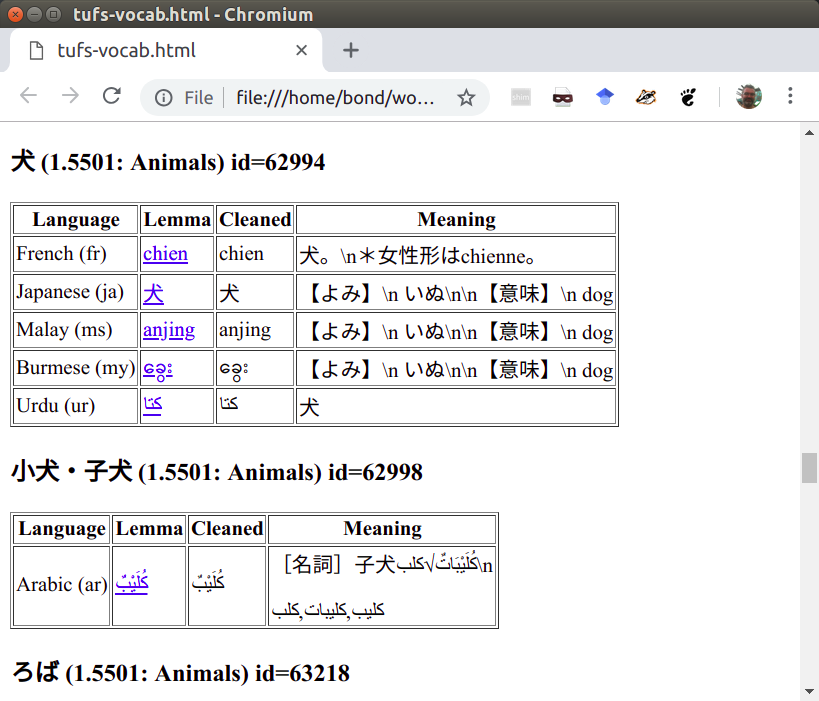
\includegraphics[width=0.9\textwidth]{inu-html.png}
  \caption{TUFs concept summary for 'dog' (and 'puppy')}
  \label{fig:tufs-inu}
\end{figure}

In addition to the columns shown in Figure~\ref{fig:linking}, there
are also columns for the Japanese and Chinese lemmas and definitions
(where available).  You can look up the wordnet synsets on the OMW
page:
\href{http://compling.hss.ntu.edu.sg/omw/cgi-bin/wn-grid.cgi?usrname=&gridmode=gridx&synset=02084071-n&lang=eng&lang2=eng}{entry
  for 02084071-n}.  You can cut and paste the synset ids
(e.g. 02084071-n) into the search window, or search for the lemma.


\subsection{Problematic cases}

The main problems with linking is when the granularity is not the
same.  For example, TUFS has a single entry for 切る \textit{kiru} with
two meanings listed ``switch off'' and ``cut''.    These link to very
different concepts in  wordnet.  In this case, you should link to both
concepts, and make a note: these should be two concepts in TUFS.

Sometimes the senses in wordnet are very fine: for today it has both 
15156001-n ``the day that includes the present moment (as opposed to
yesterday or tomorrow)'' and 15262921-n ``the present time or age''.
In this case you can link to both if you think both senses are likely
to be used in all languages.  Again, make a note as to which you think
is the best match.


% \subsubsection{Ambiguous Concept in TUFS}

% \subsubsection{}

\subsection{Errors in the resources}

If you find errors in either TUFS or wordnet, including the Japanese
and Chinese lemmas and definitions, please make a note.

For example, the Japanese wordnet has '洋犬' as an entry for the
synset for dog, but it should be a hyponym (foreign (Western) breed of
dog).

\end{document}

%%% Local Variables: 
%%% coding: utf-8
%%% mode: latex
%%% TeX-PDF-mode: t
%%% TeX-engine: xetex
%%% TeX-master: t
%%% End: 
